% !TEX TS-program = pdflatex
% !TEX encoding = UTF-8 Unicode

%%% DOCUMENT DEFINITIONS
\documentclass[11pt, french]{article} % use larger type; default would be 10pt
\usepackage[utf8]{inputenc} % set input encoding (not needed with XeLaTeX)

%%% PAGE DIMENSIONS
\usepackage{geometry} % to change the page dimensions
\geometry{a4paper} % or letterpaper (US) or a5paper or....
\geometry{margin=2cm} % for example, change the margins to 2 inches all round

%%% PACKAGES
\usepackage{graphicx} % support the \includegraphics command and options
\usepackage{booktabs} % for much better looking tables
\usepackage{array} % for better arrays (eg matrices) in maths
\usepackage{paralist} % very flexible & customisable lists (eg. enumerate/itemize, etc.)
\usepackage{verbatim} % adds environment for commenting out blocks of text & for better verbatim
\usepackage{subfig} % make it possible to include more than one captioned figure/table in a single float
\usepackage{amsmath}
\usepackage[frenchb]{babel}

\usepackage{picins,caption}
\usepackage{wrapfig}
\usepackage{url}

%%% HEADERS & FOOTERS
%\usepackage{fancyhdr} % This should be set AFTER setting up the page geometry
%\pagestyle{fancy} % options: empty , plain , fancy
% Rapport projet pluridisciplinaire : etude thermique du pont en H
% : Xavier Galzin, Stanislas Bertrand, Romain Desille, Frédéric Meslin

\title{\textsc{Projet Pluridisciplinaire} \\ Solution Numérique \\
\begin{minipage}[c][20cm][c]{15cm}
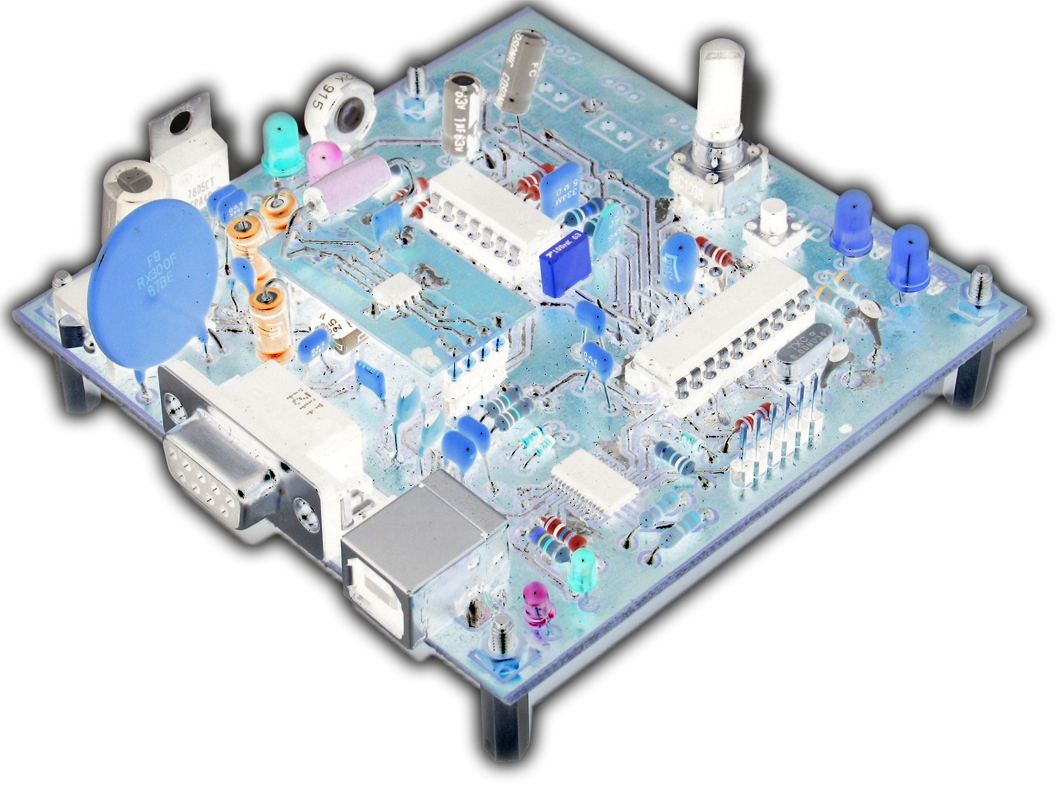
\includegraphics[width=15cm]{../Photos/CarteFrontInv.png}
\end{minipage}}
\author{Xavier GALZIN, Stanislas BERTRAND, Romain DESILLE, Frédéric MESLIN}
\date{\today}

\begin{document}
\maketitle

\pagebreak
\tableofcontents

\pagebreak
\section*{Introduction}
Xavier

\section{Communication}
	La partie communication du projet peut paraître secondaire quand on considère l'application dans sa globalité. Pour quelles raisons un luminaire aurait il besoin de communiquer avec un dispositif informatique ? L'intérêt semble limité ...

\medskip
Dans les faits, cette fonctionnalité a été implémentée dans une optique d'assistance au développement. Elle s'est avérée utile pour mettre au point l'asservissement numérique et faciliter le réglage des coefficients de la fonction de transfert du correcteur. Elle permet aussi désormais de collecter diverses informations liées à l'automatique pour analyser la qualité (stabilité) de l'asservissement. On imagine que cette liaison série ne sera pas intégrée dans le produit final, sauf si les spécifications devaient évoluer vers un appareil nécessitant de la connectivité. On peut penser à l'intégration dans un réseau domotique via des technologies Zigbee ou même au travers le Wifi.

La communication a aussi un interêt pédagogique : nous avons fait le choix d'établir un protocole dédié sur une liaison de type série prise en charge par une connection USB. Nous avons préféré cette solution à celle présentée dans la partie MCSE du projet pour plusieures raisons qui vont être détaillées.

\subsection{Choix de la liaison USB}
	
Dans l'univers de la communication péri-informatique, la liaison USB est figure souveraine. La première version de cette spécification a vue le jour en 1996 dans l'objectif de remplacer progressivement les anciennes connectiques lentes et incompatibles entre elles.

%\begin{figure}[h!]
%	\centering
%	
\includegraphics[width = 4cm]{SolutionNumerique/usb-logo.jpg} 
%	\caption{Logo USB 2.0}
%\end{figure}

\begin{wrapfigure}{r}{5cm}
	
\includegraphics[width = 4cm]{SolutionNumerique/usb-logo.jpg}
	\caption{Logo USB 2.0}
\end{wrapfigure}

\medskip
Ce document normalise à la fois : 
\medskip
\begin{itemize}
	\item un protocole complet de communication série maitre vers esclaves
	\item le matériel nécessaire pour faire transister l'information (cable, prises ...)
	\item toutes les caractéristiques électriques et mécaniques associées
	\item des classes de pilotes standards couvrant un nombre important d'applications génériques.
\end{itemize}

\medskip
Notre application étant destinée à communiquer avec un ordinateur et l'USB fournissant une classe générique de communication série équivalente à un port COM virtuel, nous avons choisi d'opter pour cette solution.

\subsection{Utilisation d'un contrôleur USB - Série}

	Afin de bénéficier de la connectique USB sans entrer dans les détails de la sous-couche de communication, nécessitant des cycles de développement lourds, deux solutions s'offraient à nous :

\medskip
\begin{enumerate}
	\item Choisir un micro-contrôleur disposant de fonctionnalités USB
	\item Utiliser un contrôleur USB externe
\end{enumerate}

\medskip
La première solution est la plus polyvalente car elle permet d'implanter n'importe quelle classe de périphérique dans le programme du micro-contrôleur en se basant sur une bibliothèque USB fournie par le constructeur. Ceci nécessite une étude approfondie de la documentation associée et la rédaction de descripteurs USBs. Etant donné l'aspect auxiliaire de la communication, ce surcroit de développement a été écarté.

La seconde solution impliquant l'ajout d'un composant externe, au détriment du coût, a été retenue pour l'aisance de développement qu'elle apporte. Cette solution clef en main convertit une liaison série TTL en provenance du micro-contrôleur en liaison USB de manière presque transparente.

\begin{figure}[h!]
	\centering
	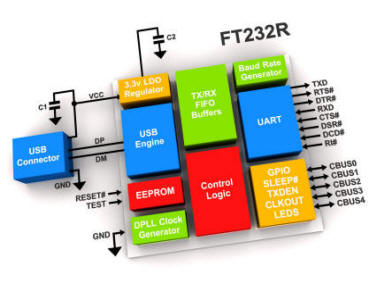
\includegraphics[width = 12cm]{SolutionNumerique/diagrammeFT232.jpg} 
	\caption{Diagramme interne du FT232}
\end{figure}

Le contrôleur circuit qui a été sélectionné est le FT232R de FTDI. Ce composant a été très simple à intégrer sur la carte du projet car il ne nécessite qu'une alimentation 5v et la liaison série pour fonctionner. De plus, il configure ses paramètres de transmission automatiquement en fonction de ceux communiqués par l'ordinateur à l'ouverture du port. Pour résumer ce composant est facile d'utilisation à défaut d'être peu couteux.

\subsection{Elaboration d'un protocole}
Dans le rapport de MCSE, nous avions présenté un protocole basique, exploitant un format de trames fixe de 3 octets consécutifs. Le premier contenant l'index de la commande et les deux suivants le corps de la donnée envoyée. Nous nous sommes rendus compte que ce protocole ne couvrait pas tous nos besoins et en particulier la possibilité de transmettre des messages d'erreurs ou de log.

\medskip
Nous avons donc programmé un autre protocole, plus évolué et plus évolutif. Celui ci est capable de transmettre plusieurs types de trames à longueur variable et d'inclure des codes de gestion d'erreur de transmission (au besoin).

\subsubsection{Configuration générale}
\noindent
Les paramètres généraux utilisés dans la transmission série sont les suivants :
\begin{description}
	\item[Taille donnée] 8 bits
	\item[Parité] Aucune parité
	\item[Bits de stops] 1 seul
	\item[Baudrate] variable de 9600 à 115200
\end{description}

\medskip
Le baudrate est variable car le micro-contrôleur dispose d'un module capable de déterminer automatiquement la vitesse de transmission de la liaison. La seule condition à respecter est l'émission du caractère ASCII "U" avant toute communication. Ce caractère correspond à un motif de niveaux logiques hauts et bas alternés qui permettent au périphérique série du micro-contrôleur de calibrer son registre prescaler pour générer le bon baudrate.

\subsubsection{Différentes trames}
\noindent
Les différentes trames disponibles sont les suivantes :
\medskip
\begin{itemize}
	\item Trame de contrôle : \\

		\begin{tabular} {|c|c|c|c|c|c|c|c|}
			\hline
			\textbf{typ} & \textbf{r/w} & \textbf{chr} & \textbf{ad4} & \textbf{ad3} & \textbf{ad2} & \textbf{ad1} & \textbf{ad0}\\
			\hline
			0 & 0 &  0 &  x &  x &  x &  x &  x \\ \hline
		\end{tabular}

		\begin{description}
			\item[typ :] type de trame (0 : données | 1 : contrôle)
			\item[r/w :] type de transfert (0 : lecture | 1 : écriture)
			\item[chr :] type de données envoyées (0 : entiers 16 bits | 1 : chaine de caractères)
			\item[ad4 ... ad0] destination de la donnée (entière) concernée (0 - 32)
		\end{description}

	\medskip
	\item Trame de donnée entière : \\

		\begin{tabular} {|c|c|c|c|c|c|c|c|c|}
			\hline
			\textbf{MSB :} & \textbf{typ} & \textbf{b06} & \textbf{b05} & \textbf{b04} & \textbf{b03} & \textbf{b02} & \textbf{b01} & \textbf{b00}\\
			\hline
			 & 0 & 0 &  0 &  0 &  d15 &  d14 &  d13 &  d12 \\ \hline
		\end{tabular}

		\begin{tabular} {|c|c|c|c|c|c|c|c|c|}
			\hline
			\textbf{MSB :} & \textbf{typ} & \textbf{b06} & \textbf{b05} & \textbf{b04} & \textbf{b03} & \textbf{b02} & \textbf{b01} & \textbf{b00}\\
			\hline
			 & 0 & 0 &  0 &  0 &  d11 &  d10 &  d09 &  d08 \\ \hline
		\end{tabular}

		\begin{tabular} {|c|c|c|c|c|c|c|c|c|}
			\hline
			\textbf{LSB : } & \textbf{typ} & \textbf{b06} & \textbf{b05} & \textbf{b04} & \textbf{b03} & \textbf{b02} & \textbf{b01} & \textbf{b00}\\
			\hline
			 & 0 & 0 &  0 &  0 &  d07 &  d06 &  d05&  d04 \\ \hline
		\end{tabular}

		\begin{tabular} {|c|c|c|c|c|c|c|c|c|}
			\hline
			\textbf{LSB : } & \textbf{typ} & \textbf{b06} & \textbf{b05} & \textbf{b04} & \textbf{b03} & \textbf{b02} & \textbf{b01} & \textbf{b00}\\
			\hline
			 & 0 & 0 &  0 &  0 &  d03 &  d02 &  d01 &  d00 \\ \hline
		\end{tabular}

		\begin{description}
			\item[typ :] type de trame (0 : données | 1 : contrôle)
			\item[d15 ... d00] valeur de la donnée 16 bits
		\end{description}

	\medskip
	\item Trame de chaine de caractères : \\

		\begin{tabular} {|c|c|c|c|c|c|c|c|}
			\hline
			\textbf{typ} & \textbf{r/w} & \textbf{log} & \textbf{ad4} & \textbf{ad3} & \textbf{ad2} & \textbf{ad1} & \textbf{ad0}\\
			\hline
			0 &  ch6 &  ch5 &  ch4 &  ch3 &  ch2 &  ch1 &  ch0 \\ \hline
		\end{tabular}

		\begin{description}
			\item[typ :] type de trame (0 : données | 1 : contrôle)
			\item[ch6 ... ch0] caractère table ASCII standard
		\end{description}

		Pour terminer l'envoi d'une chaine, il suffit d'envoyer une trame ne contenant que des zéros. Ceci correspondant à l'envoi du caractère ASCII de terminaison.

\end{itemize}

\subsection{Implantation du protocole}

\section{Interface}
Romain
\section{Changement de Puissance}
Xavier
\section{Correction Numérique}

Difference avec le rapport d'auto
-> Foh vers Zoh
-> Fréquence de travail

Questions / causes probables :
-> est-ce que le gain de l'avance de phase compte ( analogique ) ?
-> mauvais correcteur
-> mauvais modèle
-> mauvais calcul -> saturation, écretage, arondis

Utilisation d'un outils :
-> suivit des calculs via la série ( diff, avance de phase, sortie )

dernière seance
-> 1 gain du montage différentiel
-> 2 validation avec matlab de la répartition du gain ( av ph, num)
-> 3 validation avec l'asservissement numerique du mercredi du solex
-> 4 essaye d'amélioration de l'asservissement numérique


\section{Répartition des gains}
Xavier - Fred
\subsection{Correcteur Analogique}
\subsection{Correcteur Numérique}
\section*{Conclusion - Evolution}
Xavier

\end{document}

